\documentclass[]{article}
\usepackage{lmodern}
\usepackage{amssymb,amsmath}
\usepackage{ifxetex,ifluatex}
\usepackage{fixltx2e} % provides \textsubscript
\ifnum 0\ifxetex 1\fi\ifluatex 1\fi=0 % if pdftex
  \usepackage[T1]{fontenc}
  \usepackage[utf8]{inputenc}
\else % if luatex or xelatex
  \ifxetex
    \usepackage{mathspec}
  \else
    \usepackage{fontspec}
  \fi
  \defaultfontfeatures{Ligatures=TeX,Scale=MatchLowercase}
\fi
% use upquote if available, for straight quotes in verbatim environments
\IfFileExists{upquote.sty}{\usepackage{upquote}}{}
% use microtype if available
\IfFileExists{microtype.sty}{%
\usepackage{microtype}
\UseMicrotypeSet[protrusion]{basicmath} % disable protrusion for tt fonts
}{}
\usepackage[margin=1in]{geometry}
\usepackage{hyperref}
\hypersetup{unicode=true,
            pdftitle={BLP Simulation},
            pdfauthor={Nutcha Wattanachit},
            pdfborder={0 0 0},
            breaklinks=true}
\urlstyle{same}  % don't use monospace font for urls
\usepackage{graphicx,grffile}
\makeatletter
\def\maxwidth{\ifdim\Gin@nat@width>\linewidth\linewidth\else\Gin@nat@width\fi}
\def\maxheight{\ifdim\Gin@nat@height>\textheight\textheight\else\Gin@nat@height\fi}
\makeatother
% Scale images if necessary, so that they will not overflow the page
% margins by default, and it is still possible to overwrite the defaults
% using explicit options in \includegraphics[width, height, ...]{}
\setkeys{Gin}{width=\maxwidth,height=\maxheight,keepaspectratio}
\IfFileExists{parskip.sty}{%
\usepackage{parskip}
}{% else
\setlength{\parindent}{0pt}
\setlength{\parskip}{6pt plus 2pt minus 1pt}
}
\setlength{\emergencystretch}{3em}  % prevent overfull lines
\providecommand{\tightlist}{%
  \setlength{\itemsep}{0pt}\setlength{\parskip}{0pt}}
\setcounter{secnumdepth}{0}
% Redefines (sub)paragraphs to behave more like sections
\ifx\paragraph\undefined\else
\let\oldparagraph\paragraph
\renewcommand{\paragraph}[1]{\oldparagraph{#1}\mbox{}}
\fi
\ifx\subparagraph\undefined\else
\let\oldsubparagraph\subparagraph
\renewcommand{\subparagraph}[1]{\oldsubparagraph{#1}\mbox{}}
\fi

%%% Use protect on footnotes to avoid problems with footnotes in titles
\let\rmarkdownfootnote\footnote%
\def\footnote{\protect\rmarkdownfootnote}

%%% Change title format to be more compact
\usepackage{titling}

% Create subtitle command for use in maketitle
\providecommand{\subtitle}[1]{
  \posttitle{
    \begin{center}\large#1\end{center}
    }
}

\setlength{\droptitle}{-2em}

  \title{BLP Simulation}
    \pretitle{\vspace{\droptitle}\centering\huge}
  \posttitle{\par}
    \author{Nutcha Wattanachit}
    \preauthor{\centering\large\emph}
  \postauthor{\par}
      \predate{\centering\large\emph}
  \postdate{\par}
    \date{12/2/2019}

\usepackage{booktabs}
\usepackage{longtable}
\usepackage{array}
\usepackage{multirow}
\usepackage{wrapfig}
\usepackage{float}
\usepackage{colortbl}
\usepackage{pdflscape}
\usepackage{tabu}
\usepackage{threeparttable}
\usepackage{threeparttablex}
\usepackage[normalem]{ulem}
\usepackage{makecell}
\usepackage{xcolor}

\usepackage{booktabs}
\usepackage{tabularx}
\usepackage{hyperref}
\usepackage{multicol}
\usepackage{longtable}
\usepackage{array}
\usepackage{multirow}
\usepackage{wrapfig}
\usepackage{float}
\usepackage{colortbl}
\usepackage{pdflscape}
\usepackage{tabu}
\usepackage{threeparttable}
\usepackage{threeparttablex}
\usepackage{makecell}
\usepackage{xcolor}

\begin{document}
\maketitle

\hypertarget{ensemblepooling-methods}{%
\section{Ensemble/pooling Methods}\label{ensemblepooling-methods}}

\hypertarget{tlp}{%
\subsection{TLP}\label{tlp}}

Traditional linear pool finds optimal weights that maximmizes the
likelihood of \(f(y)=\sum_{i=1}^k w_if_i(y)\).

\hypertarget{blp}{%
\subsection{BLP}\label{blp}}

BLP finds \(\alpha\), \(\beta\), and weights that maximize the
likelihood of

\[g_{\alpha,\beta}=(\sum_{i=1}^k w_if_i(y))b_{\alpha,\beta}(\sum_{i=1}^k w_iF_i(y)).\]

BLP Example: To obtain \(\alpha\), \(\beta\), and the weights for all
component models, train the BLP model on half of the data. Then, use
\(\alpha\), \(\beta\), and the weights from training to apply to the
data held out for testing.

\hypertarget{bias-corrected-tlp-bctlp}{%
\subsection{Bias-corrected TLP (bcTLP)}\label{bias-corrected-tlp-bctlp}}

This method corrects for bias of the component models, and then use the
traditional method to generate the ensemble. The difference between this
and the traditional TLP is that the component models inputted in bcTLP
are bias-corrected. The bias correction method used is simple linear
regression (Raftery, 2005). By regressing \(y\) against the forecast
output, we obtain the intercept and coefficient of each component,

\[g_i(y)=\alpha_i+\beta_if_i(y)\].

and the final ensemble is

\[g(y)=\sum_{i=1}^k w_ig_i(y)\].

\hypertarget{bias-corrected-blp-bcblp}{%
\subsection{Bias-corrected BLP (bcBLP)}\label{bias-corrected-blp-bcblp}}

This method also corrects for bias of the component models using linear
regression, and then use the BLP method to generate the ensemble. The
final ensemble is

\[g_{\alpha,\beta}=(\sum_{i=1}^k w_ig_i)b_{\alpha,\beta}(\sum_{i=1}^k w_iG_i(y)).\]

\hypertarget{blp-with-non-central-parameternblp}{%
\subsection{BLP with Non-central
Parameter(nBLP)}\label{blp-with-non-central-parameternblp}}

nBLP finds \(\alpha\), \(\beta\), non-central parameter \(\lambda\), and
weights that maximize the likelihood of

\(g_{\alpha,\beta,\lambda}=(\sum_{i=1}^k w_if_i(y))b_{\alpha,\beta}(\sum_{i=1}^k w_iF_i(y)).\)

nBLP process: To obtain \(\alpha\), \(\beta\), \(\lambda\), and the
weights for all component models, train the nBLP model on half of the
data. Then, use \(\alpha\), \(\beta\), \(\lambda\), and the weights from
training to apply to the data held out for testing.

\hypertarget{component-wise-blp-cblp}{%
\subsection{Component-wise BLP (cBLP)}\label{component-wise-blp-cblp}}

This is the extension of the traditional BLP. We beta-transform each of
the cumulative distribution functions of the component models. This is
done by finding \(\alpha\) and \(\beta\) that maximize the likelihood of

\[
\begin{aligned}
G_{i,\alpha_i,\beta_i} &= B_{\alpha_i,\beta_i}[F_i(y)]\\
g_{i,\alpha_i,\beta_i} &= f_i(y) \times b_{\alpha_i,\beta_i}[F_i(y)]
\end{aligned}
\]

Then, to obtain \(\alpha\), \(\beta\), and the weights for 21 models, we
apply BLP on the beta-transformed components:

\[
\begin{aligned}
G_{\alpha,\beta} &= B_{\alpha,\beta}\Big[\sum_{i=1}^k w_iB_{\alpha_i,\beta_i}(F_i(y))\Big]\\
g_{\alpha,\beta} &= \Big(\sum_{i=1}^k w_ib_{i,\alpha_i,\beta_i}(F_i(y))f_i(y)  \Big)b_{\alpha,\beta} \Big(\sum_{i=1}^k w_iB_{i,\alpha_i,\beta_i}(F_i(y))\Big)
\end{aligned}
\]

cBLP - Part 1: For each component model, train over all observations to
get \(\alpha_i\) and \(\beta_i\). Then, apply \(\alpha_i\) and
\(\beta_i\) to beta-transform the CDF. This ends the component-wise
part.

cBLP Part 2: Apply the usual BLP process on the beta-transformed
component models to get the BLP ensemble.

\hypertarget{componentwise-bias-corrected-componentwise-recalibrated-blp-cbcblp}{%
\subsection{Componentwise Bias-Corrected \& Componentwise Recalibrated
BLP
(cbcBLP)}\label{componentwise-bias-corrected-componentwise-recalibrated-blp-cbcblp}}

This method corrects for bias of the component models and also
recalibrate them using beta transform. Then the BLP method is used to
generate the ensemble.

\clearpage

\hypertarget{simulation-studies}{%
\section{Simulation studies}\label{simulation-studies}}

The data generating process for the observation \(Y\) in the regression
model is

\[
Y=X_0+a_1X_1+a_2X_2+a_3X_3+\epsilon, \epsilon\sim(0,1)
\]

where \(a_1,a_2,\) and \(a_3\) are real constants that vary across
different simulation studies, and \(X_0,X_1,X_2,X_3,\) and \(\epsilon\)
are independent, standard normal random variables. The individual
predictive densities have partial access of the above set of covariates.
\(f_1\) has access to only \(X_0\) and \(X_1\), \(f_2\) has access to
only \(X_0\) and \(X_2\), and \(f_3\) has access to only \(X_0\) and
\(X_3\). We want to combine \(f_1,f_2,\) and \(f_3\) to predict \(Y\).
In this setup, \(X_0\) represent shared information, while other
covariates represent information unique to each individual model.

We estimate the pooling/combination formulas on a random sample
\({(f_{1i} , f_{2i} , f_{3i}, Y_i) : i = 1,..., n}\) of size
\(n = 50,000\) and evaluate on an independent test sample of the same
size.

\hypertarget{scenario-1-calibrated-components-baseline-scenario.}{%
\subsection{Scenario 1: calibrated components (Baseline
scenario).}\label{scenario-1-calibrated-components-baseline-scenario.}}

In this scenario, \(a_1 = a_2 = 1\) and \(a_3 = 1.1\), so that \(f_3\)
is a more concentrated, sharper density forecast than \(f_1\) and
\(f_2\) (Gneiting and Ranjan (2013)) and they are defined as follows:

\[
\begin{aligned}
f_1&=\text{N}(X_0+a_1X_1,1+a^2_2+a^2_3)\\
f_2&=\text{N}(X_0+a_2X_2,1+a^2_1+a^2_3)\\
f_3&=\text{N}(X_0+a_3X_3,1+a^2_1+a^2_2)\\
\end{aligned}
\]

\begin{table}[!h]
\caption{\label{tab:unnamed-chunk-3}Model Parameters and Log Score}

\centering
\begin{tabular}[t]{lrrrrrr}
\toprule
  & w1 & w2 & w3 & alpha & beta & ncp\\
\midrule
\rowcolor{gray!6}  TLP & 0.271 & 0.264 & 0.465 & NA & NA & NA\\
BLP & 0.301 & 0.295 & 0.404 & 1.465 & 1.469 & NA\\
\rowcolor{gray!6}  bcTLP & 0.272 & 0.264 & 0.464 & NA & NA & NA\\
bcBLP & 0.301 & 0.296 & 0.403 & 1.477 & 1.477 & NA\\
\rowcolor{gray!6}  nBLP & 0.301 & 0.295 & 0.404 & 1.452 & 1.483 & 0.076\\
\addlinespace
cBLP & 0.300 & 0.296 & 0.405 & 1.459 & 1.460 & NA\\
\rowcolor{gray!6}  cbcBLP & 0.301 & 0.296 & 0.403 & 1.469 & 1.469 & NA\\
\bottomrule
\end{tabular}
\centering
\begin{tabular}[t]{lrr}
\toprule
  & Training & Test\\
\midrule
\rowcolor{gray!6}  f1 & -1.998 & -2.004\\
f2 & -1.999 & -2.006\\
\rowcolor{gray!6}  f3 & -1.965 & -1.969\\
TLP & -1.907 & -1.912\\
\rowcolor{gray!6}  BLP & -1.864 & -1.872\\
\addlinespace
bcTLP & -1.906 & -1.911\\
\rowcolor{gray!6}  bcBLP & -1.861 & -1.870\\
nBLP & -1.864 & -1.872\\
\rowcolor{gray!6}  cBLP & -1.864 & -1.872\\
cbcBLP & -1.862 & -1.870\\
\bottomrule
\end{tabular}
\end{table}

\begin{figure}[H]

{\centering 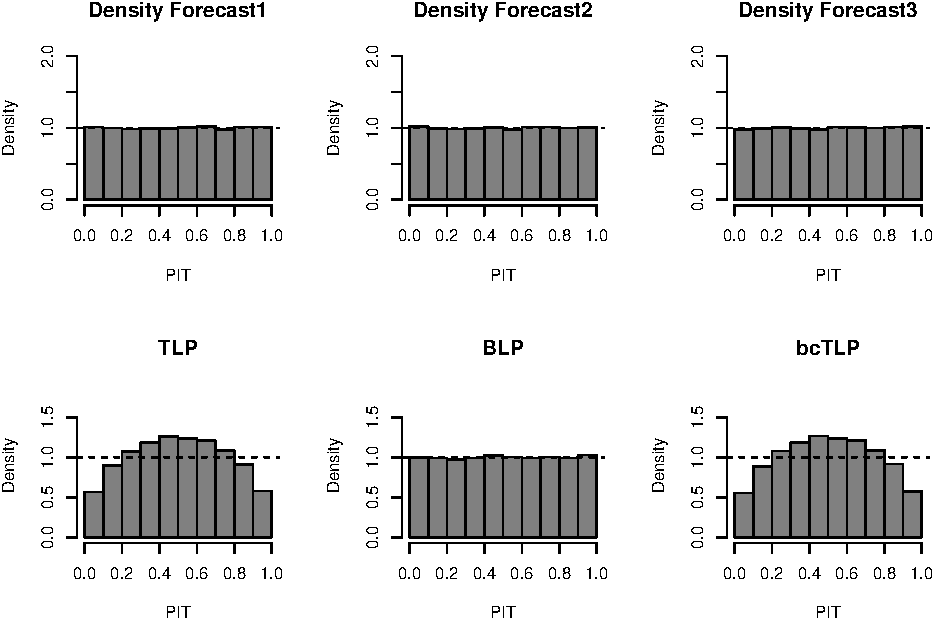
\includegraphics{Newest_BLPsim_files/figure-latex/unnamed-chunk-4-1} 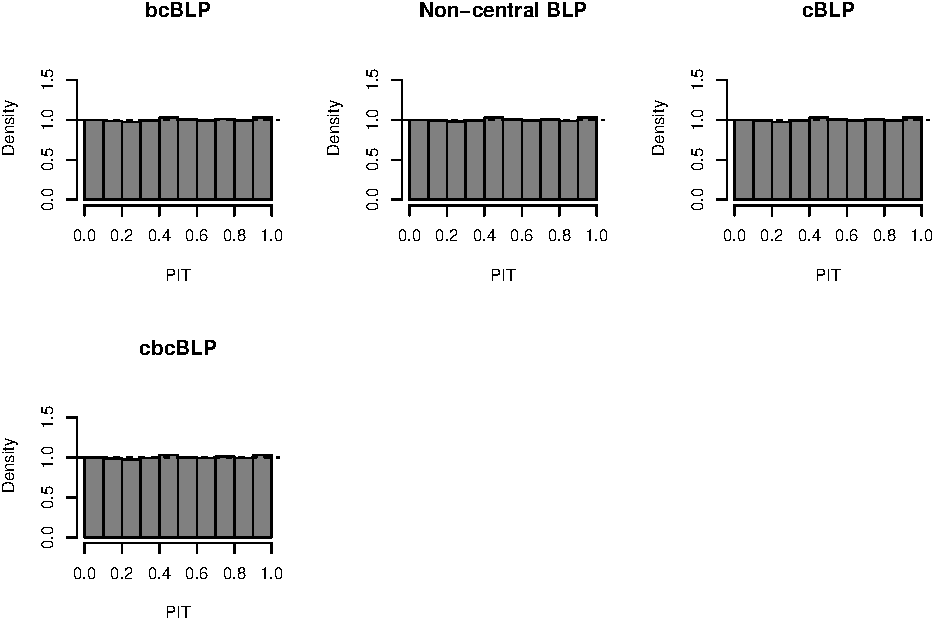
\includegraphics{Newest_BLPsim_files/figure-latex/unnamed-chunk-4-2} 

}

\end{figure}

\clearpage

\hypertarget{scenario-2-biased-forecast-scenario}{%
\subsection{Scenario 2: Biased forecast
scenario}\label{scenario-2-biased-forecast-scenario}}

In this scenario, \(a_1 = a_2 = 1\) and \(a_3 = 1.1\), and we add
\(N(2,1)\) to the mean of \(f_1\) so that it is a biased forecast. The
models are defined as follows:

\[
\begin{aligned}
f_1&=\text{N}(X_0+a_1X_1+N(2,1),1+a^2_2+a^2_3)\\
f_2&=\text{N}(X_0+a_2X_2,1+a^2_1+a^2_3)\\
f_3&=\text{N}(X_0+a_3X_3,1+a^2_1+a^2_2)\\
\end{aligned}
\]

\begin{center}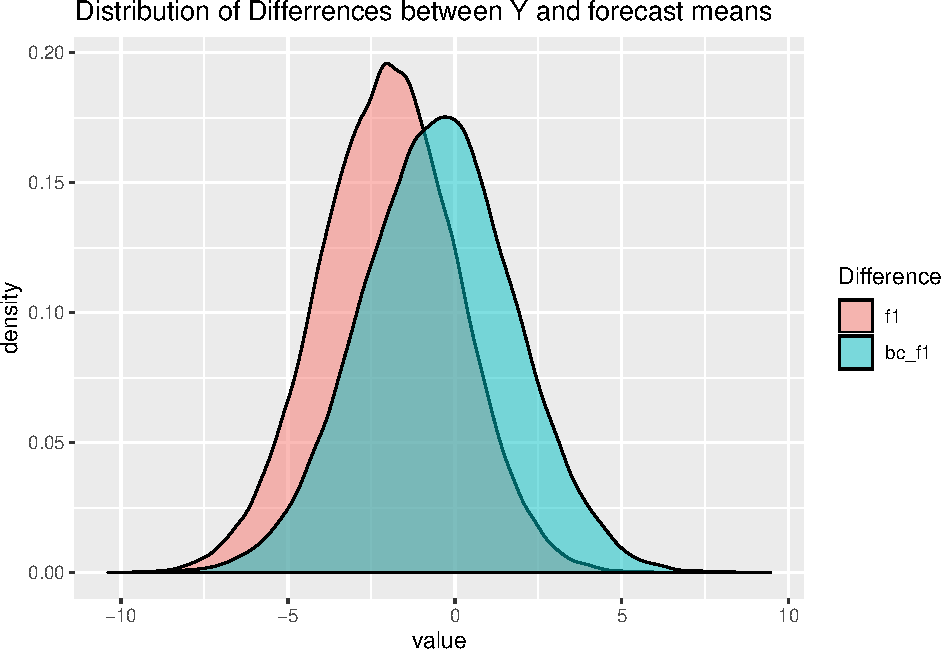
\includegraphics[width=0.6\linewidth,height=0.6\textheight]{Newest_BLPsim_files/figure-latex/unnamed-chunk-6-1} \end{center}

\begin{table}[!h]
\caption{\label{tab:unnamed-chunk-8}Model Parameters and Log Score}

\centering
\begin{tabular}[t]{lrrrrrr}
\toprule
  & w1 & w2 & w3 & alpha & beta & ncp\\
\midrule
\rowcolor{gray!6}  TLP & 0.000 & 0.000 & 1.000 & NA & NA & NA\\
BLP & 0.140 & 0.391 & 0.469 & 1.420 & 1.676 & NA\\
\rowcolor{gray!6}  bcTLP & 0.005 & 0.417 & 0.579 & NA & NA & NA\\
bcBLP & 0.088 & 0.411 & 0.500 & 1.372 & 1.373 & NA\\
\rowcolor{gray!6}  nBLP & 0.138 & 0.390 & 0.472 & 1.309 & 1.822 & 0.653\\
\addlinespace
cBLP & 0.183 & 0.381 & 0.436 & 1.510 & 1.518 & NA\\
\rowcolor{gray!6}  cbcBLP & 0.133 & 0.386 & 0.481 & 1.398 & 1.399 & NA\\
\bottomrule
\end{tabular}
\centering
\begin{tabular}[t]{lrr}
\toprule
  & Training & Test\\
\midrule
\rowcolor{gray!6}  f1 & -2.788 & -2.777\\
f2 & -1.998 & -2.004\\
\rowcolor{gray!6}  f3 & -1.965 & -1.969\\
TLP & -1.965 & -1.969\\
\rowcolor{gray!6}  BLP & -1.884 & -1.888\\
\addlinespace
bcTLP & -1.917 & -1.921\\
\rowcolor{gray!6}  bcBLP & -1.888 & -1.893\\
nBLP & -1.883 & -1.888\\
\rowcolor{gray!6}  cBLP & -1.967 & -1.971\\
cbcBLP & -1.895 & -1.900\\
\bottomrule
\end{tabular}
\end{table}

\begin{figure}[H]

{\centering 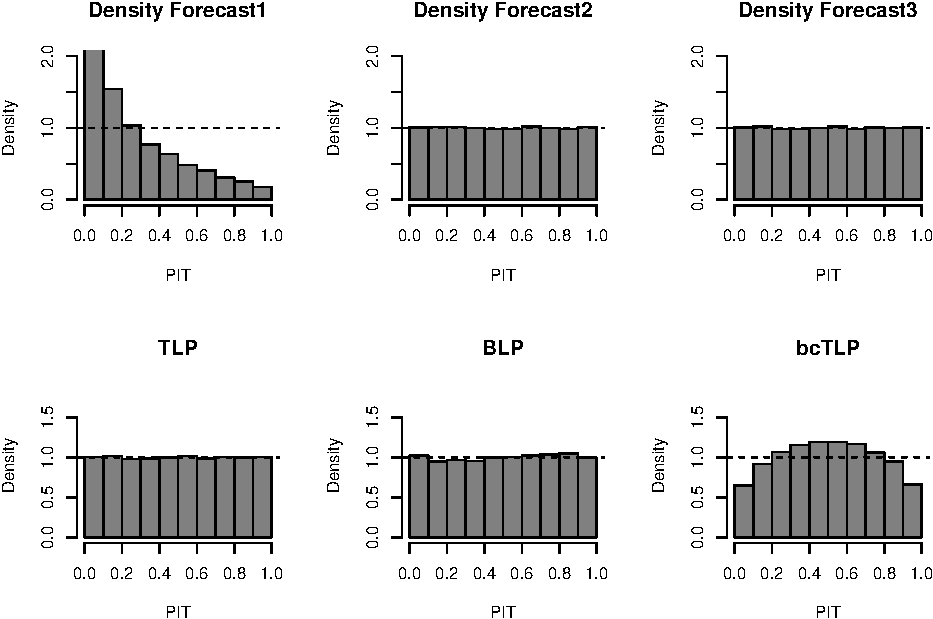
\includegraphics{Newest_BLPsim_files/figure-latex/unnamed-chunk-9-1} 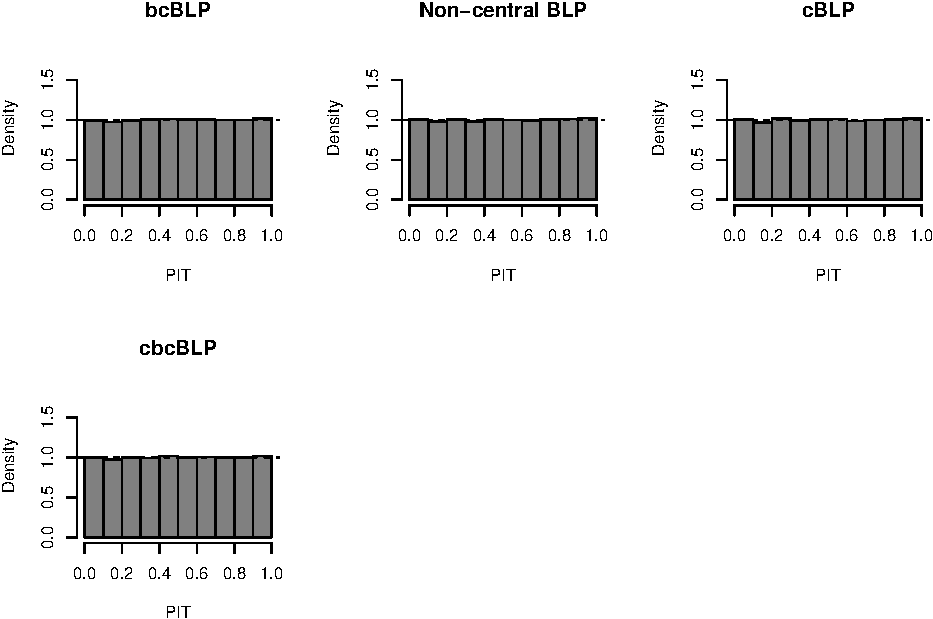
\includegraphics{Newest_BLPsim_files/figure-latex/unnamed-chunk-9-2} 

}

\end{figure}

\hypertarget{scenario-3-higher-variance-forecast-scenario}{%
\subsection{Scenario 3 : Higher variance forecast
scenario}\label{scenario-3-higher-variance-forecast-scenario}}

We modified the standard deviation of the first density forecast by
adding a constant of 2 as follows:

\[
\begin{aligned}
f_1&=\text{N}(X_0+a_1X_1,1+a^2_2+a^2_3+2)\\
f_2&=\text{N}(X_0+a_2X_2,1+a^2_1+a^2_3)\\
f_3&=\text{N}(X_0+a_3X_3,1+a^2_1+a^2_2)\\
\end{aligned}
\]

\begin{table}[!h]
\caption{\label{tab:unnamed-chunk-12}Model Parameters and Log Score}

\centering
\begin{tabular}[t]{lrrrrrr}
\toprule
  & w1 & w2 & w3 & alpha & beta & ncp\\
\midrule
\rowcolor{gray!6}  TLP & 0.013 & 0.411 & 0.576 & NA & NA & NA\\
BLP & 0.327 & 0.288 & 0.385 & 1.658 & 1.668 & NA\\
\rowcolor{gray!6}  bcTLP & 0.013 & 0.412 & 0.575 & NA & NA & NA\\
bcBLP & 0.327 & 0.289 & 0.384 & 1.668 & 1.668 & NA\\
\rowcolor{gray!6}  nBLP & 0.327 & 0.288 & 0.385 & 1.654 & 1.672 & 0.02\\
\addlinespace
cBLP & 0.204 & 0.357 & 0.439 & 1.443 & 1.444 & NA\\
\rowcolor{gray!6}  cbcBLP & 0.204 & 0.357 & 0.439 & 1.448 & 1.448 & NA\\
\bottomrule
\end{tabular}
\centering
\begin{tabular}[t]{lrr}
\toprule
  & Training & Test\\
\midrule
\rowcolor{gray!6}  f1 & -2.051 & -2.053\\
f2 & -1.998 & -2.004\\
\rowcolor{gray!6}  f3 & -1.965 & -1.969\\
TLP & -1.918 & -1.921\\
\rowcolor{gray!6}  BLP & -1.864 & -1.869\\
\addlinespace
bcTLP & -1.917 & -1.921\\
\rowcolor{gray!6}  bcBLP & -1.863 & -1.868\\
nBLP & -1.864 & -1.869\\
\rowcolor{gray!6}  cBLP & -1.866 & -1.871\\
cbcBLP & -1.865 & -1.870\\
\bottomrule
\end{tabular}
\end{table}

\begin{figure}[H]

{\centering 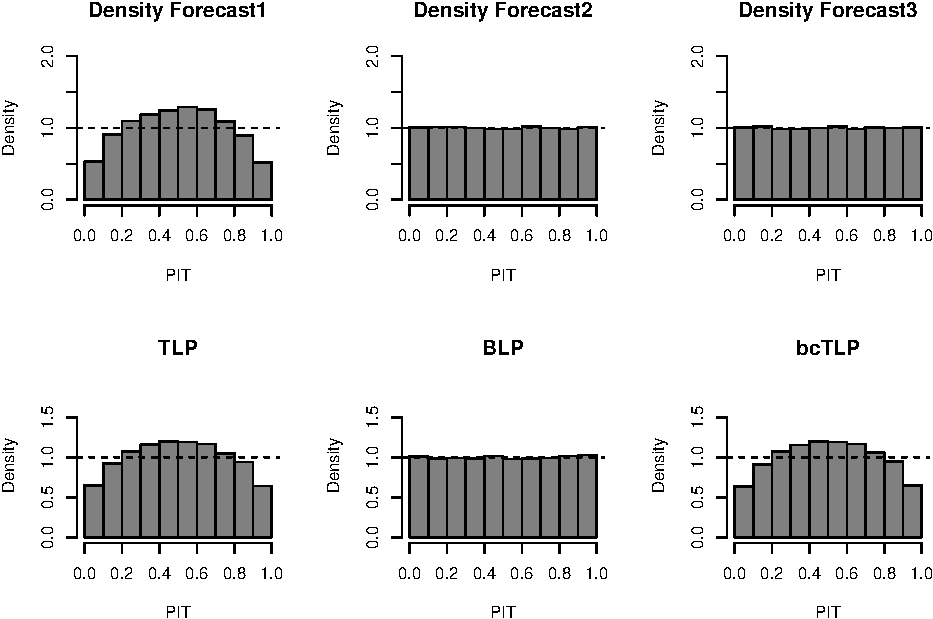
\includegraphics{Newest_BLPsim_files/figure-latex/unnamed-chunk-13-1} 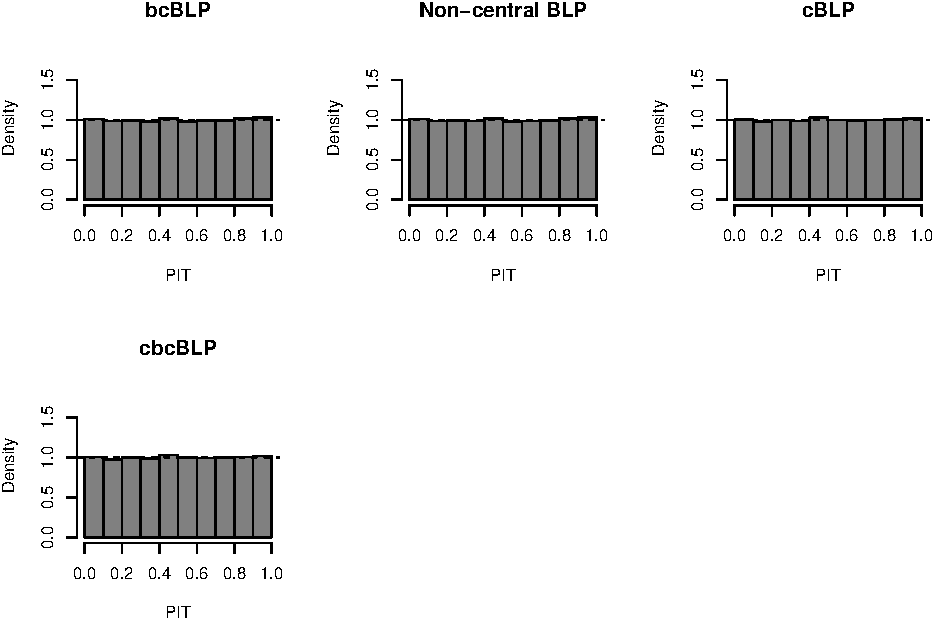
\includegraphics{Newest_BLPsim_files/figure-latex/unnamed-chunk-13-2} 

}

\end{figure}

\clearpage

\hypertarget{scenario-4-biased-higher-variance-forecast-scenario}{%
\subsection{Scenario 4 Biased + higher variance forecast
scenario}\label{scenario-4-biased-higher-variance-forecast-scenario}}

In this scenario, \(a_1 = a_2 = 1\) and \(a_3 = 1.1\), but we modified
the standard deviation of the first and second density forecast as
follows:

\[
\begin{aligned}
f_1&=\text{N}(X_0+a_1X_1+N(2,1),1+a^2_2+a^2_3)\\
f_2&=\text{N}(X_0+a_2X_2,1+a^2_1+a^2_3+2)\\
f_3&=\text{N}(X_0+a_3X_3,1+a^2_1+a^2_2)\\
\end{aligned}
\]

\begin{center}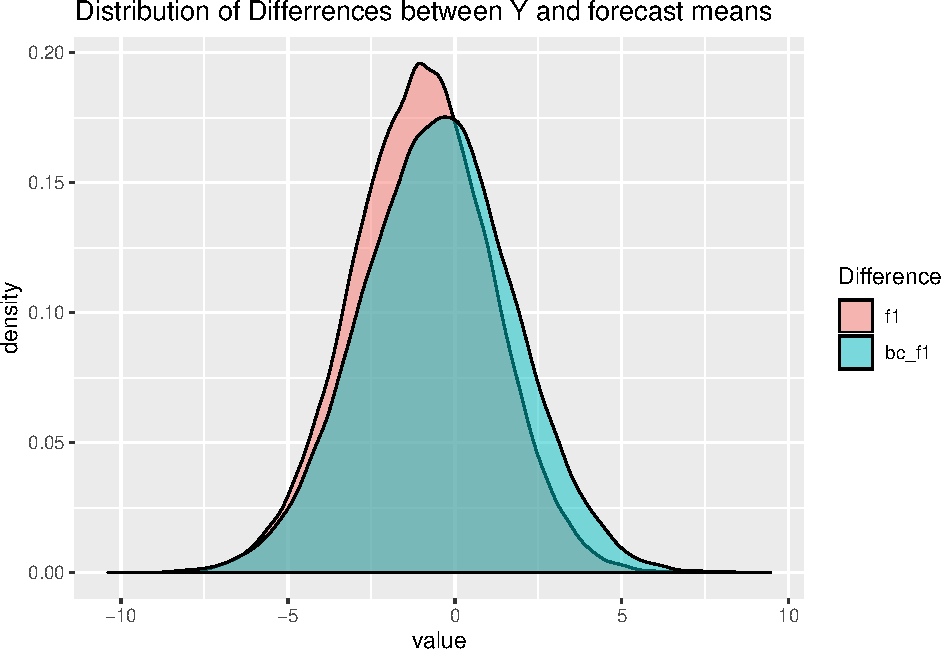
\includegraphics[width=0.6\linewidth,height=0.6\textheight]{Newest_BLPsim_files/figure-latex/unnamed-chunk-15-1} \end{center}

\begin{table}[!h]
\caption{\label{tab:unnamed-chunk-17}Model Parameters and Log Score}

\centering
\begin{tabular}[t]{lrrrrrr}
\toprule
  & w1 & w2 & w3 & alpha & beta & ncp\\
\midrule
\rowcolor{gray!6}  TLP & 0.000 & 0.000 & 1.000 & NA & NA & NA\\
BLP & 0.161 & 0.414 & 0.425 & 1.660 & 1.832 & NA\\
\rowcolor{gray!6}  bcTLP & 0.130 & 0.150 & 0.720 & NA & NA & NA\\
bcBLP & 0.085 & 0.453 & 0.461 & 1.639 & 1.639 & NA\\
\rowcolor{gray!6}  nBLP & 0.160 & 0.414 & 0.426 & 1.648 & 1.846 & 0.068\\
\addlinespace
cBLP & 0.249 & 0.264 & 0.487 & 1.524 & 1.528 & NA\\
\rowcolor{gray!6}  cbcBLP & 0.205 & 0.281 & 0.514 & 1.401 & 1.401 & NA\\
\bottomrule
\end{tabular}
\centering
\begin{tabular}[t]{lrr}
\toprule
  & Training & Test\\
\midrule
\rowcolor{gray!6}  f1 & -2.317 & -2.310\\
f2 & -2.050 & -2.054\\
\rowcolor{gray!6}  f3 & -1.965 & -1.969\\
TLP & -1.965 & -1.969\\
\rowcolor{gray!6}  BLP & -1.878 & -1.882\\
\addlinespace
bcTLP & -1.942 & -1.945\\
\rowcolor{gray!6}  bcBLP & -1.888 & -1.893\\
nBLP & -1.878 & -1.882\\
\rowcolor{gray!6}  cBLP & -1.915 & -1.920\\
cbcBLP & -1.905 & -1.910\\
\bottomrule
\end{tabular}
\end{table}

\begin{figure}[H]

{\centering 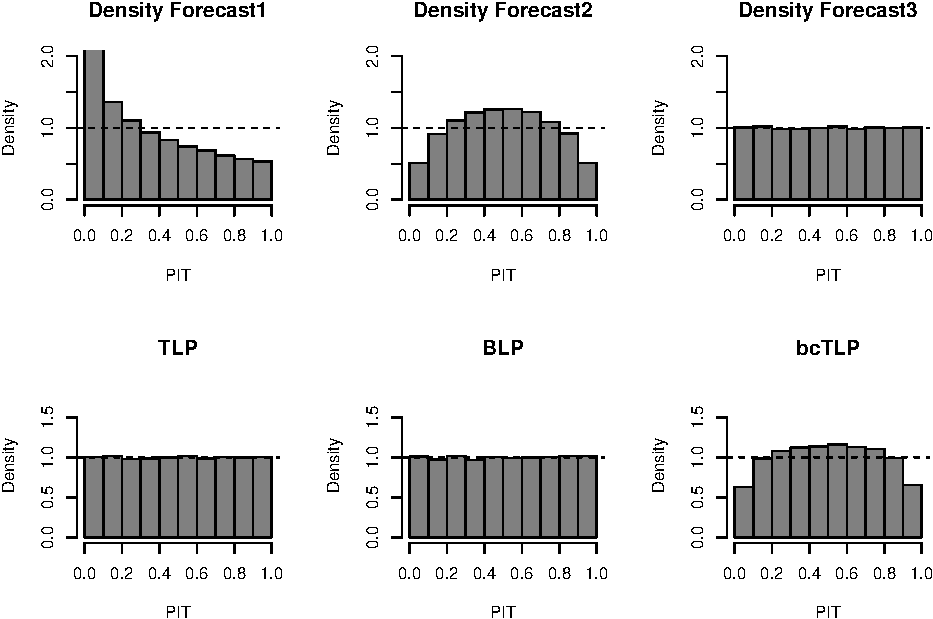
\includegraphics{Newest_BLPsim_files/figure-latex/unnamed-chunk-18-1} 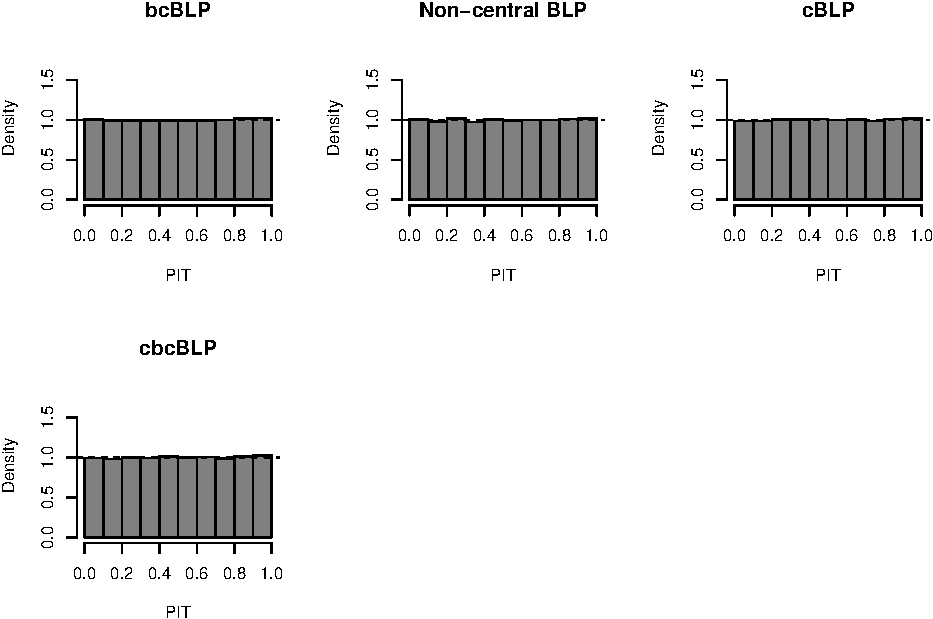
\includegraphics{Newest_BLPsim_files/figure-latex/unnamed-chunk-18-2} 

}

\end{figure}

\clearpage


\end{document}
